\documentclass[12pt]{article}\usepackage[]{graphicx}\usepackage[]{color}
%% maxwidth is the original width if it is less than linewidth
%% otherwise use linewidth (to make sure the graphics do not exceed the margin)
\makeatletter
\def\maxwidth{ %
  \ifdim\Gin@nat@width>\linewidth
    \linewidth
  \else
    \Gin@nat@width
  \fi
}
\makeatother

\definecolor{fgcolor}{rgb}{0.345, 0.345, 0.345}
\newcommand{\hlnum}[1]{\textcolor[rgb]{0.686,0.059,0.569}{#1}}%
\newcommand{\hlstr}[1]{\textcolor[rgb]{0.192,0.494,0.8}{#1}}%
\newcommand{\hlcom}[1]{\textcolor[rgb]{0.678,0.584,0.686}{\textit{#1}}}%
\newcommand{\hlopt}[1]{\textcolor[rgb]{0,0,0}{#1}}%
\newcommand{\hlstd}[1]{\textcolor[rgb]{0.345,0.345,0.345}{#1}}%
\newcommand{\hlkwa}[1]{\textcolor[rgb]{0.161,0.373,0.58}{\textbf{#1}}}%
\newcommand{\hlkwb}[1]{\textcolor[rgb]{0.69,0.353,0.396}{#1}}%
\newcommand{\hlkwc}[1]{\textcolor[rgb]{0.333,0.667,0.333}{#1}}%
\newcommand{\hlkwd}[1]{\textcolor[rgb]{0.737,0.353,0.396}{\textbf{#1}}}%

\usepackage{framed}
\makeatletter
\newenvironment{kframe}{%
 \def\at@end@of@kframe{}%
 \ifinner\ifhmode%
  \def\at@end@of@kframe{\end{minipage}}%
  \begin{minipage}{\columnwidth}%
 \fi\fi%
 \def\FrameCommand##1{\hskip\@totalleftmargin \hskip-\fboxsep
 \colorbox{shadecolor}{##1}\hskip-\fboxsep
     % There is no \\@totalrightmargin, so:
     \hskip-\linewidth \hskip-\@totalleftmargin \hskip\columnwidth}%
 \MakeFramed {\advance\hsize-\width
   \@totalleftmargin\z@ \linewidth\hsize
   \@setminipage}}%
 {\par\unskip\endMakeFramed%
 \at@end@of@kframe}
\makeatother

\definecolor{shadecolor}{rgb}{.97, .97, .97}
\definecolor{messagecolor}{rgb}{0, 0, 0}
\definecolor{warningcolor}{rgb}{1, 0, 1}
\definecolor{errorcolor}{rgb}{1, 0, 0}
\newenvironment{knitrout}{}{} % an empty environment to be redefined in TeX

\usepackage{alltt}
\usepackage{amssymb}
\usepackage{natbib}
\usepackage{algorithm,algpseudocode}
\usepackage{color}
\usepackage{hyperref}
%\usepackage{fullpage}
%\VignetteIndexEntry{Simulation Report} 
%\VignetteDepends{evolMC,knitr} 
%\VignetteEngine{knitr::knitr}
\usepackage{setspace}

\usepackage[nolists]{endfloat}
\renewcommand{\efloatseparator}{} %multiple floats per page
\renewcommand{\floatplace}[1]{} %no [about here] marker text
\DeclareDelayedFloat{algorithm}[aaa]{Algorithms} %endfloat algorithms


\newcommand{\grady}[1]{\marginpar{#1--Grady}}
\newcommand{\bx}{\mathbf x}
\newcommand{\bt}{\mathbf t}
\newcommand{\X}{\mathcal X}
\newcommand{\U}{\mathcal U}
\newcommand{\Exp}{\mathcal E}
\newcommand{\needcite}{{\color{red}[citation needed]}}
\newcommand{\ret}{{\bf return} }

\algdef{SE}[WP]{Wp}{EndWp}[1]{{\bf with prob}\ #1\ }{\algorithmicend\
  {\bf w/prob}}%
\algdef{Ce}[OW]{WP}{Ow}{EndWp}{{\bf otherwise}\ }%




\title{evolMC: a package for Monte-Carlo simulation}
\author{W Burchett \and E Roualdes \and G Weyenberg}
\IfFileExists{upquote.sty}{\usepackage{upquote}}{}


\begin{document}
\maketitle
\doublespacing

\begin{abstract}
  Sampling from multi-modal target distributions proves difficult for basic MCMC methods.  Borrowing from the evolutionary based algorithms of optimization theory, \cite{Liang:2000} introduced evolutionary Monte Carlo (EMC).  EMC begins with parallel tempering and then adds to it a step in which sequences intelligently evolve by learning from each other.  A comparative simulation highlights the effectiveness of EMC over other sampling methods.
\end{abstract}

%%    \section{Introduction}
\vspace{1cm}
\label{sec:introduction}
Markov Chain Monte Carlo methods, as exemplified by the classic
\cite{Metropolis:1953} and \cite{Hastings:1970} algorithms, are an
important tool in contemporary statistics.  However, the basic
algorithms often do not work well in situations where the distribution of
interest possesses multiple modes. Several extensions have been
suggested to alleviate this problem. In this paper we explore two such
algorithms, Parallel Tempering \citep{swendsen1986replica}, and a further
extension, the Evolutionary algorithms of \cite{Liang:2000}.

Parallel tempering  simulates multiple sequences from a ``heated''
target distribution, and then proposes to exchange information between
the chains according to the Metropolis rule. This helps to encourage a
more thorough global search of the support space. \citep{Liang:2011}
Evolutionary Monte Carlo (EMC) builds upon parallel tempering by
blending with it ideas taken from evolutionary biology. In particular,
the Chromosomal crossovers that are observed in Meiosis are
simulated. Such crossovers are thought to be an important component of
the success of sexual reproduction.



Iterations of the EMC algorithm consist of three operations: mutation,
crossover, and exchange. Each type of operation makes a specific type
of modification to the current population, and the change is carried
forward to the next generation with a probability governed by a
Metropolis-type rule.\citep{Liang:2011}

In general terms, a mutation operation adds noise to the current
population. This can be analogous to a basic random walk type
proposal, but more elaborate methods have been proposed. A crossover
operator consists of randomly selecting two individuals and generating
replacement individuals by somehow mixing the parent values, analogous
to the Chromosomal crossovers that sometimes occur during Meiosis.  An
exchange step proposes a switch of two randomly selected individuals
without switching their associated temperatures.


In the remainder of this paper we compare the performance of the EMC
algorithm to parallel tempering and a na\"ive Metropolis sampler in
the context of a 3 dimensional distribution with 20 modes.  Section
two describes in greater detail the algorithms used and the simulation
setup.  While results of the simulation are presented and discussed in
sections \ref{sec:results} and \ref{sec:discussion}.

\setcounter{section}{1}
\section{Methods}
\label{sec:methods}
The target distribution for our study is a 20-part mixture of
trivariate Gaussian distributions. Each part of the mixture is
$\mathcal{N}_3(\mu_i, 0.1I_3)$, and each vector $\mu_i$ is located
uniformly in $[-10,10]\times[-10,10]\times[-10,10].$ This distribution
possesses numerous modes that are separated by relatively large
regions of low probability, making it challenging for a basic
Metropolis sampler to mix between the modes.

\subsection{Algorithms}
\label{sec:algorithms}
The discussion of population based Monte Carlo methods necessarily
begins by introducing some terminology. The following recounts the
terminology given in Chapter 5 of \cite{Liang:2011}: We wish to sample
from a distribution $f(x|t) \propto \exp\{ -H(x)/t \}$, where $t\ge 1$
is called the \emph{temperature} and $H(x)$, called the \emph{fitness
  function}, corresponds to the negative log-density of $x$, up to a
constant. A \emph{population} $\mathbf{x}$ consists of $N$
\emph{individuals} $x_i$, $i = 1, \ldots, N$, and we also define an
associated set of temperatures $\bt = (t_1,\ldots,t_N)$. ($x_i \in
\mathbb{R}^d$ and the $t_i$ are in descending order.) Each individual
$x_i$ is independently sampled from the distribution $f_i(x_i) \propto
f(x_i|t_i)$.  For any such distribution, the \emph{partition function}
$Z(t)= \int_\X f(x|t) dx$ is the inverse of the normalizing
constant. The \emph{Boltzmann distribution} of the population $\bx$ is
the product of the individual distributions, $f(\bx) \propto \exp \{
-\sum_{i=1}^N H(x_i)/ t_i \}$, with $Z(\bt) := \prod_{i=1}^N Z(t_i)$
as the inverse of the normalizing constant.

The EMC algorithm we have implemented is described briefly in
Algorithms \ref{alg:emc}--\ref{alg:exchange}.  The mutate step uses a
simple random-walk approach, where the variance of the noise
distribution depends on the temperature of the individual being
modified.  The crossover we used is a simple single-splice version,
where the parents are selected with weights based on their fitness.


\begin{algorithm}
  \caption{Evolutionary Monte Carlo}
  \label{alg:emc}
  \footnotesize
  \begin{algorithmic}
  \Procedure{EMC}{} \Wp{$p_m$} \Comment{$p_m$ is the \emph{mutation probability}.}  \State \Call{Mutate}{} \Ow \State \Call{Crossover}{}
    \EndWp
    \State \Call{Exchange}{}
    \EndProcedure
\end{algorithmic}
\end{algorithm}


\begin{algorithm}
  \caption{A random-walk \emph{mutation}.}
  \label{alg:mutate}
  \footnotesize
  \begin{algorithmic}
  \Procedure{Mutate}{} \State Copy the current population to $x$.  \ForAll{individuals in $x$} \State $y \gets \mathcal N_d(x_i,t_i \sigma^2I)$ \Wp{$\min\{1,\exp(\cdots)\}$} \State $x_i \gets y$
    \EndWp
    \EndFor
    \State Set current population to $x$.
    \EndProcedure
\end{algorithmic}
\end{algorithm}

\begin{algorithm}
  \caption{The fitness-weighted \emph{crossover}.}
  \label{alg:crossover}
  \footnotesize
  \begin{algorithmic}
  \Procedure{Crossover}{} \State Copy the current population to $x$.  \ForAll {individuals in $x$} \State $w_i \gets \exp(-H(x_i))$
    \EndFor
    \State Select $k$ uniformly from $\{1\colon d\}.$ \State Select $i$ from $\{1\colon N\}$ with weights proportional to $\{w_\cdot\}$.  \State Select $j$ uniformly from $\{1\colon N\} \backslash \{i\}.$ \State In $x$, swap elements $k\colon d$ of individuals $i$ and $j$.  \Wp {$\min\{1, \exp(-H(x_i)/t_i +H(x_j)/t_j+\cdots)\}$} \State Set the current population to $x$.
    \EndWp
    \EndProcedure
\end{algorithmic}
\end{algorithm}

\begin{algorithm}
  \caption{The \emph{exchange} attempts to swap individuals between neighboring temperature states.}
  \label{alg:exchange}
  \footnotesize
  \begin{algorithmic}
  \Procedure{Exchange}{} \State Copy the current population to $x$.  \State Select $i$ uniformly from $\{1\colon N\}$.  \State Select $j$ uniformly from $\{i\pm 1\}\cap\{1\colon N\}$.  \State Swap individuals $i,j$ of $x$.  \Wp{$\min\{1,\exp(-H(x_i)/t_i +H(x_j)/t_j)\}$} \State Set the current population to $x$.
    \EndWp
    \EndProcedure
\end{algorithmic}
\end{algorithm}

\subsection{Simulations}
\label{sec:methods-simulations}
The algorithms described have several tuning parameters that the user
must supply. We ran simulations in an attempt to come to a qualitative
understanding of the effects that these tuning parameters have on the
performance of the Markov Chain. We ran chains on all combinations of
options described below.

The choice of mutator distribution: Gaussian noise with variance
dependent on the temperature, or a uniform proposal with no
temperature dependance.  We tested three different temperature
ladders: $(1,5)$, $(1,2, 4, 8, 15)$, and $(1,5,15,30,50)$. (There is a
great deal of freedom in the selection of the temperature ladder, but
we attempted to study the effect of an insufficient number of
temperature settings, as well as the effect of changing the spacing of
temperature levels.)  The mutation/crossover selection probabilities:
$p_m \in \{0.1, 0.5, 0.9, 1.0\}$. Note that $p_m = 1.0$ is equivalent to
parallel tempering.

The chains were run for a $20,000$ iterations. This is not nearly a
long enough run to accurately estimate the mixing proportions, however
it should allow us to get a sense of how easily the chains explore the
space. If a mode is not explored by this point, then the chain is
clearly mixing quite poorly. However if all modes are being visited in
this amount of time then the average dwelling time per mode is at most
approximately $1000$ iterations, which is not a shockingly large number.
\section{Results}
\label{sec:results}

\subsection{Software}
\label{sec:software}

We present the R package evolMC, which is a framework for doing
Markov-Chain Monte Carlo simulations. The evolMC package includes
implementations of several MCMC algorithms, including
Metropolis-Hastings, Gibbs, parallel tempering, and the evolutionary
updating methods. The package is available from
\url{http://github.com/grady/evol-mc/}.

The package aims to provide a general framework for constructing a
chain, leaving it up to the user to provide the pieces specific to the
problem. The user must first define a \emph{state object} and then
implement a number of functions which act on this state object. In
many traditional cases this state object can simply be a vector of
reals, but any R object (e.g. a phylogenetic tree object defined by a
3rd-party package) can be used. This generality departs from many
existing R MCMC packages, which enforce vector- or array-type
structures for the random elements in question.

The functions provided by evolMC will eventually produce a
\emph{chain} object, which is simply an R list where each element is
an instance of the state object. A function is provided to convert
this object into a {\tt coda::mcmc.list} object. The evolMC package
includes a vignette demonstrating a few basic use cases, with example
code.


The main job of the user of evolMC is to define a few basic functions
which can interact in specified ways with whatever object is selected
to represent states of the chain. For example, the user will often
need to implement a function which evaluates a log-density for a given
state. Using the routines provided by evolMC, one will then manipulate
these functions, eventually producing a function which implements some
desired MCMC algorithm.


\subsection{Simulations}
\label{sec:simulations}

In the simulations discussed in the previous section, the best
criterion to assess the various methods and tuning parameters was the
number of modes the chain was able to sample from.  Figure
\ref{scatterplot} contains a plot of the states observed in select
situations. The points are layered so that chains that found more
modes are behind those which found only a few modes. Table \ref{table}
displays a count of the modes found for a subset of the scenarios
tested. 

In terms of methods, the multivariate sampler generally only finds a
single mode.  Parallel tempering and evolutionary Monte Carlo were
comparable, depending on the tuning parameters.  More temperatures
being included in the temperature ladder led to more modes being
sampled from, as chains were more easily able to move around the
entire space.  In addition, using the Gaussian proposal with a
variance weighted by the temperature for the mutation operation
produced better results than using a uniform proposal with fixed
support.

The most surprising and informative result concerns the probability of
mutation or crossover (the additional operation introduced in the
evolutionary MC method).  Lower probabilities for the crossover
operation (and therefore higher probabilities for the mutation
operation) resulted in more modes of the target distribution being
sampled from.  In fact, for this problem parallel tempering produced
samples just as good or better than the evolutionary Monte Carlo
method did.

\begin{figure}
  \centering
  \caption{Scatterplot of states realized by selected tuning parameter
    settings.}
  \label{scatterplot}
  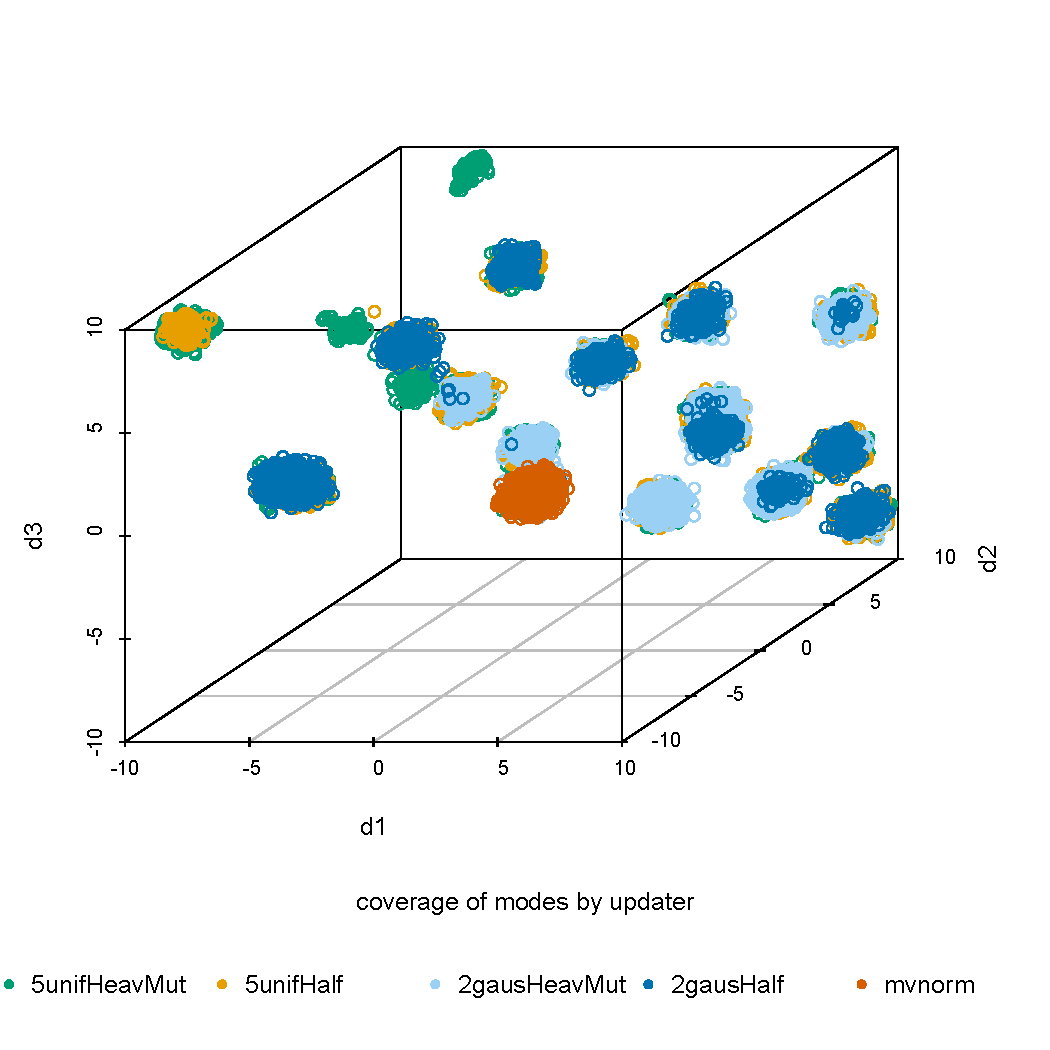
\includegraphics[width=\textwidth]{figure/final_plot.png}
\end{figure}


\begin{table}
  \centering
  \begin{tabular}{llcc}
    \hline\hline
    Temps & Mutator & $p_m$ & Modes \\ 
    \hline
    two & Gaussian & 0.1 & 2 \\ 
    two & Gaussian & 0.9 & 12 \\ 
    two & Gaussian & 0.5 & 13 \\ 
    two & Gaussian & 1 & 14 \\ 
    five.wide & Gaussian & 0.1 & 17 \\ 
    five & Gaussian & 0.1 & 18 \\ 
    five & Gaussian & 0.5 & 20 \\ 
    five.wide & Gaussian & 0.5 & 20 \\ 
    five & Gaussian & 0.9 & 20 \\ 
    five.wide & Gaussian & 0.9 & 20 \\ 
    five & Gaussian & 1 & 20 \\ 
    five.wide & Gaussian & 1 & 20 \\ 
    \hline\hline
  \end{tabular}
    \caption{Number of modes discovered by the chain for selected tuning parameter combinations.}
  \label{table}
\end{table}

\section{Discussion}
\label{sec:discussion}

Evolutionary Monte Carlo adds an additional operation, crossover, onto
the parallel tempering algorithm, which \cite{Liang:2011} claims
allows EMC to more fully explore the target distribution's space.
However, our findings in this situation are at odds to those of Liang's.

In almost all five-tuple temperature scenarios, both EMC and parallel
tempering were able to find almost every mode; the exceptions to this
rule all employed the uniform mutation proposals.  However, the
remainder of our simulations clearly show that for this target
distribution parallel tempering is sufficient to fully explore the
sample space, provided a suitable temperature ladder is chosen. The
crossover operation does not appear to significantly improve the
mixing of the chain.

The crossover that we implemented for this simulation study is perhaps
the simplest example of a crossover procedure, and indeed
\cite{Liang:2011} suggests a few more complicated ones. Further work
is warranted to explore the performance of these more complicated
crossover options. The problem of automated temperature selection is
also discussed, and implementation of these methods is a next step in
improving the usability of {\tt evolMC}.


%% BIBLIOGRAPHY HERE
\bibliography{refs} \bibliographystyle{named}

\appendix

\section{evolMC}
\label{sec:evolmc}
The evolMC package includes a vignette demonstrating a few basic use cases, with example code. Here we briefly discuss the architectural vision underlying the package and a few of the most important functions.

evolMC was designed to be as flexible as possible, and hence it operates on a quite abstract level. It is written in a very functional style of programming; most of the important functions in evolMC accept functions as arguments and return new functions. An important goal was for the user to be free to use whatever object they wish to represent a realization of the random element in question. This departs from many existing R MCMC packages, which require vector- or array-type structures for the random elements in question.

The main job of the user of evolMC is to define a few basic functions which can interact in specified ways with whatever object is selected to represent states of the chain. For example, the user will often need to implement a function which evaluates a log-density for a given state. Using the routines provided by evolMC, one will then manipulate these functions, eventually producing a function which implements some desired MCMC algorithm.

The core function in evolMC is \texttt{iterate(n,f,x)}. This function is also among the least interesting, because it simply creates a list where the $(k+1)$-th element is $f^{k}(x)$. (Function exponentiation means iterated application here.) If the provided function {\tt f} is ``carefully selected'' then the resulting chain might have ``desirable properties''. Of course, we are likely interested in the case where the desirable property in question is that the resulting list represents a sample from some target distribution. Most other functions in the package exist to help one in constructing a function {\tt f} with specific desirable properties.

Perhaps the most basic MCMC algorithm is the Gibbs sampler. Suppose we want to sample from $[x,y]$. If we can sample from $[x|y]$ and $[y|x]$, then we can implement a Gibbs sampler. To do this one need only implement functions {\tt rxy} and {\tt ryx}, which do the respective sampling. These functions should accept the current state as their first argument, and return a new state object with the relavant changes made.

Once one has these functions, the gibbs function can be used to produce a new updating function which will implement the Gibbs algorithm. The basic signature is {\tt gibbs(...)}. The ...  argument allows one to provide any number of updating functions; in our case we have two, {\tt rxy} and {\tt ryx}. The result of {\tt gibbs(rxy,ryx)} is a new ``carefully selected'' function with signature \texttt{function(state)} which acts as a Gibbs updater. If called repeatedly (e.g. by iterate) it will alternate between using {\tt rxy} and {\tt ryx} to update the state.\footnote{The sequential choice of updating functions is the default mode of operation for the function returned by {\tt gibbs}. It can also stochastically select an updating function according to provided weights.}

A second important algorithm is the Metropolis algorithm. The function {\tt metropolis} helps one to construct an updating function which implements Metropolis-Hastings. To use this function one must first implement: the log-density function for the target distribution ({\tt ln.d}); a proposal generator function ({\tt r.prop}); and (if required) a log-density function for the proposal generator ({\tt ln.d.prop}). A call {\tt metropolis(ln.d, r.prop, ln.d.prop)} will return a ``carefully selected'' function (with signature {\tt function(state)}), which implements the Metropolis-Hastings scheme you have defined.

These three basic building blocks can be used to construct a surprising number of more advanced MCMC algorithms, and indeed many of the more advanced algorithms provided by evolMC are constructed using only these pieces.
\end{document}
